%Compiled with TexLive + Visual Studio
\documentclass[11pt,letterpaper]{article}

\usepackage{fullpage}
\usepackage[top=2cm, bottom=4.5cm, left=2.5cm, headsep=24pt, right=2.5cm]{geometry}
\usepackage{amsmath,amsthm,amsfonts,amssymb,amscd}
\usepackage{lastpage}
\usepackage{enumerate}
\usepackage{fancyhdr}
\usepackage{mathrsfs}
\usepackage{xcolor}
\usepackage{graphicx}
\usepackage{listings}
\usepackage{booktabs}
\usepackage{amsmath}
\usepackage[utf8]{inputenc}
\usepackage{physics}
\usepackage[colorlinks=true, allcolors=blue]{hyperref}
\usepackage{siunitx}
\usepackage{bm}
\usepackage{float}
\usepackage{pdfpages}

\usepackage{minted}

\let\oldvec=\vec
\renewcommand{\vec}[1]{\oldvec{\mathbf{#1}}}
\def\doubleunderline#1{\underline{\underline{#1}}}

\def\spvec#1{\left(\vcenter{\halign{\hfil$##$\hfil\cr \spvecA#1;;}}\right)}
\def\spvecA#1;{\if;#1;\else #1\cr \expandafter \spvecA \fi}

\renewcommand{\\}{\bigskip}

\newenvironment{qns}[1]
    {\begin{center}
    \begin{tabular}{|p{0.9\textwidth}|}
    \hline
    \begin{center}
        \textbf{#1}\\[1ex]
    \end{center}

    }
    { 
    \\\\\hline
    \end{tabular} 
    \end{center}
    }

\newtheorem{sol}{Solution}[subsection]
  
\newtheorem{thm}{Theorem}

\renewcommand*{\l}{\left(}
\renewcommand*{\r}{\right)}
\newcommand{\partialt}{\frac{\partial}{\partial t}}
\newcommand{\expectation}[1]{\left\langle #1 \right\rangle}
\newcommand{\brakett}[3]{\left\langle#1\left|#2\right|#3\right\rangle}
\newcommand{\partialf}[3]{\frac{\partial^{#3} #1}{\partial #2^{#3}}}
\newcommand{\lbar}{\left|}
\newcommand{\rbar}{\right|}
\renewcommand*{\b}[1]{\mathbf{#1}}
\def\matrix#1{\underline{\underline{#1}}}






\title{Wavepacket Propagation Program (w/ Dr Nadav Avidor)}
\author{Lorenzo Basso, Jack Lee, Matthew Zhang, Feiyang Chen}
\date{April 2020}

\begin{document}

\maketitle

\tableofcontents


\pagestyle{fancy}
\renewcommand{\subsectionmark}[1]{\markright{#1}{}}
\fancyhead[C]{Version 5.0}
\fancyfoot[C]{\thepage}% \fancyfoot[R]{\thepage}
\fancyhead[L]{\leftmark}
\fancyhead[R]{\rightmark}

\newpage

\section{Wavepacket Propagation Introduction}
\subsection{About}

The Wavepacket propagation project is an extension of a Part III project by Ocean Haghighi-Daly. It is a 3D working version of a Working attempt at a Split-Operator method of wavepacket propagation. 


\subsection{Prerequisites}

To begin with, a computer with a CUDA compatible GPU (\href{https://developer.nvidia.com/cuda-gpus#compute}{List of compatible GPUs}) is required.The MEX/CUDA dependent files have already been compiled for an x64 Linux and x64 Windows system with CUDA 10.1 compatibility. However, it is potentially necessary to install a CUDA/C++ compiler depending on the CUDA capability your GPU has.\\

\textbf{Installation Guides:}

\begin{itemize}
    \item \href{https://developer.nvidia.com/cuda-downloads?target_os=Windows&target_arch=x86_64}{Latest CUDA Package Download} (If you believe you don't need to follow the installation guides as the Windows install is reasonably simple)
    \item \href{https://docs.nvidia.com/cuda/cuda-installation-guide-microsoft-windows/index.html}{Windows Installation Guide}
    \item \href{https://docs.nvidia.com/cuda/cuda-installation-guide-linux/index.html}{Linux Installation Guide}
    \item \href{https://docs.nvidia.com/cuda/cuda-installation-guide-mac-os-x/index.html}{Mac OS X Installation Guide}
\end{itemize}

These guides also include the relevant instructions to install CUDA/C++ compilers for your relevant OS. If for some reason the documentation is too tedious, we will (maybe) try to provide a simplified version that produces functionality in the \hyperref[sec:compilerinstall]{Appendix}\\

\textbf{Setup MEXCUDA Compiler}\\

\textbf{Windows:}\\

For Windows, Visual Studio must be installed with the Desktop Development Package for C++ installed. If the user has MinGW compiler installer for previous MEX compile operators, then it may be necessary to change compilers. This is because MinGW is incompatible with MEXCUDA operations. This can be done by running

\begin{minted}{matlab}
    mex -setup C++
\end{minted}

Which will output something like the following:

\begin{minted}{matlab}
    MEX configured to use 'Microsoft Visual C++ 2019' for C++ language compilation.

    'To choose a different C++ compiler, select one from the following':
    MinGW64 mex -setup:'C:\PATHTO\mexopts\mingw64_g++.xml' C++
    MSVS_2019 mex -setup:'C:\PATHTO\mexopts\msvcpp2019.xml' C++ 
\end{minted}

\begin{center}
    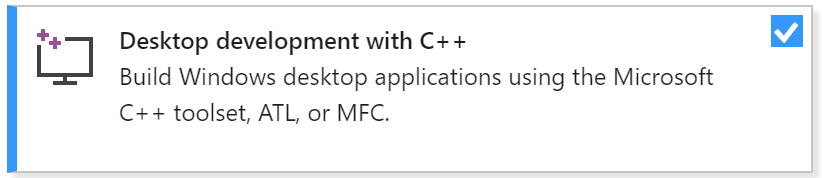
\includegraphics[width = 0.6\textwidth]{Windows_Compiler.png}
\end{center}

\textbf{Linux:}\\

For a Linux system, the CUDA installation should come with the corresponding NVCC compiler for MEXCUDA. GCC (The standard C++ compiler) is a prerequisite to installing CUDA, and is also necessary for code compilation.

\bigskip

\textbf{The required Matlab Toolboxes for the program to function are as follows:}
\begin{itemize}
    \item Parallel Computing Toolbox
    \item Bioinformatics Toolbox
\end{itemize}

\section{Usage}

\subsection{Initialization/WavePacketPropagation\_Beta4\_2} 

All variables are in SI units. SetupSIUnits.m initializes global variables used in picoscale wavefunction propagation:

\begin{align*}
    \textbf{hBar} &= 1.054571800 \times 10^{-34} Js\\
    \textbf{c} &= 299792458 m/s\\
    \textbf{eV} &= 1.6021766208 \times 10^{-19} J\\
    \textbf{amu} &=  1.660539040 \times 10^{-27} kg\\
    \textbf{A} &= 1.00 \times 10^{-10} m\\
    \textbf{ps} &= 1.00 \times 10^{-12} s
\end{align*}

\textbf{lx}, \textbf{ly}, \textbf{lz} define the length of the box in which you want the wavefunction to propagate, while \textbf{nx, ny, nz} denote the grid sizing (how finely you want to splice up essentially). Grid sizing also determines how much memory is used (approximately $nx \times ny \times nz$ bits).\\

\textbf{RealTimePlotting} displays each figure at the time intervals determined by \textbf{numGfxToSave}. Having this setting on also saves the figures when \textbf{SavingSimulationRunning = true}. It is greatly advised to either change \textbf{numGfxToSave} to 1 or set \textbf{RealTimePlotting} to false as it will greatly improve the simulation speed.\\

\textbf{SavingSimulationRunning} will create a folder under "SavedSimulation" (unless otherwise specified by the user by changing \textbf{saveLocation}) and save the matlab arrays of the wavefunction while the program is running. With \textbf{RealTimePlotting} set as true, the figures shown will also be saved. The number of pictures saved is dependent on \textbf{numGfxToSave}. \textbf{numGfxToSave} breaks up the total iteration time into equally spaced blocks of time. It will also save the initialization data, and additionally, the final wavefunction as a matlab data file.\\

\textbf{SavingSimulationEnd} only saves the final wavefunction, as well as the initialization data. This can be used if the propagation of the wavefunction is not as important.\\

\textbf{DisplayAdsorbateAnimation} shows the motion of the adsorbates fed in. This setting is useful if you're feeding a custom potential+path to ensure that it is phrased correctly.\\

\textbf{savingBrownianPaths} will save the randomly generated path to a txt file \textbf{Browniefile} which can then be fed back to be used as a custom potential later.\\

\textbf{propagationMethod} dictates the propagation method used for the program. The methods are as follows:

\begin{enumerate}
    \item Runge-Kutta method of Order 4
    \item Split Operator of Order 2
    \item Split Operator of Order 3 with K split
    \item Split Operator of Order 3 with V split
    \item Split Operator of Order 3 with V split, Time dependent
    \item MEXCUDA while loop with Split Operator $O(dt^3)$ with Vsplit, Time dependent (This is the fastest implementation of CUDA)
    \item Split Operator of Order 3 with V split, Time dependent in Matlab and CUDA (Primarily to compare the two methods, will output the average difference in the Psi tensor for each)
    \item Matlab while loop with CUDA Split Operator Order 3, V Split, Time dependent (slower than method 6)
\end{enumerate}

\bigskip

\textbf{numAdsorbates} determines the number of adsorbates on the scatter surface. !!!Currently, it appears that using \textbf{custompaths = true} requires that the \# of adsorbates is equal to the \# used in the custom path!!! (will likely be patched out hopefully)\\

\textbf{custompaths} is the file you feed with a custom potential and path for the adsorbates. The instructions are further detailed \hyperref[sec:custompaths]{below}.\\

\textbf{I do not really know what these next three do precisely so will have to converse with others to discuss}\\

\textbf{decayType}  1 = exponential repulsive. 2 = Morse attractive. 3 = Morse-like (needs alpha parameter input too!). 4=custom\\
    
\textbf{potfile} for 4, text file containing floats for real and imaginary part of potential, seperated by lz. potential should be high to prevent tunelling over cyclic boundary\\

\textbf{zOffset} Shift entire V away from boundary to stop Q.Tunneling through V or to make custom potential go all the way to the surface\\

\subsection{Setup Folder}

It is likely that the only file in here that needs to be changed at a user level will be \textbf{SetupInitialWavefunction.m}. If an alternative wavepacket is necessitated, it is preferable to add an alternative generating function rather than change the existing ones (\textbf{})

\label{sec:custompaths}
\subsection{Custom Paths and Potentials}
Functionality to include custom adsorbate paths and potentials was added by Jack Lee.

\begin{enumerate}
    \item Custom potential: this allows you to specify a custom potential profile in the Z direction. To apply this, set decaytype to 4 and specify a .txt file (in beta4\_2) as a string in potfile. This should contain several numbers separated by spaces (or new lines) which are the values for the potential in Joules in each cell of the simulation out from the corrugation function (+zoffset), i.e. the values are separated by a distance of lz/nz. The potential is zero for all z not specified by the file. Zoffset should have a negative value, and can be used to extend the potential back from the gaussians to the surface, as if zoffset is 0 the area between the surface and the gaussian peaks will have 0 potential. The potential specified should be very high near the surface to prevent the wavepacket from getting past it, because the propagation algorithm leads to cyclic boundary conditions so any psi that reaches the end will appear at the other side, which is non-physical.
    \item Custom paths: this allows you to specify the paths that adsorbates take, rather than having them be generated randomly. To enable this, set custompaths to true and specify in pathfile a text file (in beta4\_2) formatted as follows: the first entry on each line should be a time, then for each adsorbate there should be its x position and then its y position at that time, separated by spaces. There can be any number of times, as long as the first is $\leq$ tStart and the last is $\geq$ tFinish, and they’ll be interpolated to get the paths. 
    \item Saving paths: this allows you to save the randomly generated paths adsorbates take this time in the simulation. It doesn’t do anything if custom paths is on. To enable it, set savingBrownianPaths to true and name a .txt file in Browniefile, which will be overwritten or created in beta4\_2. This saves the paths in the same format as Custom paths reads them, with one line for each timestep of the simulation. These files can later be read by custom paths to reproduce this simulation (and could be used to vary the potential, detail etc.), although there is a small error introduced here so that the final psi from the custom paths simulation is slightly different to that of the original. Two custom paths simulations from the same source will be the same, however.
\end{enumerate}



\section{Appendix}

\subsection{CUDA + Compiler Install}

\label{sec:compilerinstall}
\subsubsection{Windows}
Installation for Windows is reasonably straightfoward. It requires first to download the \href{https://developer.nvidia.com/cuda-downloads?target_os=Windows&target_arch=x86_64}{Latest CUDA Package Download} and run the relevant executable file.\\

\begin{center}
    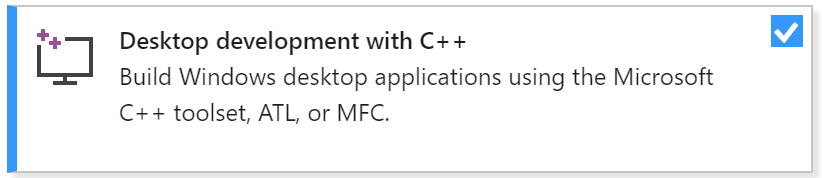
\includegraphics[width = 0.6\textwidth]{Windows_Compiler.png}
\end{center}

Next, Visual Studio must be installed with the Desktop Development Package for C++ installed. If the user has MinGW compiler installer for previous MEX compile operators, then it may be necessary to change compilers. This is because MinGW is incompatible with MEXCUDA operations. This can be done by running

\begin{minted}{matlab}
    mex -setup C++
\end{minted}

Which will output something like the following:

\begin{minted}{matlab}
    MEX configured to use 'Microsoft Visual C++ 2019' for C++ language compilation.

    'To choose a different C++ compiler, select one from the following':
    MinGW64 mex -setup:'C:\PATHTO\mexopts\mingw64_g++.xml' C++
    MSVS_2019 mex -setup:'C:\PATHTO\mexopts\msvcpp2019.xml' C++ 
\end{minted}


\subsubsection{Linux}
CUDA installation for Linux is significantly more annoying than Windows. As the installs for different distros can vary fairly significantly, the best suggestion I have is for the user to follow the instructions in the installation guides.\\

The corresponding CUDA install should come with the NVCC compiler necessary to compile the MEXCUDA files.


\subsection{Ocean Report}

The report is displayed on the next pages
\includepdf[pages=-]{Ocean_report.pdf}


\subsection{Test}
\end{document}
